\normalfalse \difficiletrue \tdifficilefalse
\correctionfalse

%\UPSTIidClasse{11} % 11 sup, 12 spé
%\newcommand{\UPSTIidClasse}{12}

\exer{Barrière Sympact $\star\star$ \label{DYN:04:B2:12:14}}
\setcounter{question}{0}\marginnote{\xpComp{DYN}{04}}%\UPSTIcompetence{B2-12}
\index{Compétence B2-13}\index{Compétence DYN-04}
\index{Barrière Sympact}
\ifcorrection
\else
\marginnote{\textbf{Pas de corrigé pour cet exercice.}}
\fi
\ifprof
\else
Soit le mécanisme suivant. On a $\vect{AC}=H\vect{j_0}$ et $\vect{CB}=R\vect{i_1}$. De plus, 
$H=\SI{120}{mm}$, $R=\SI{40}{mm}$ $BI=\SI{10}{mm}$.

\begin{marginfigure}
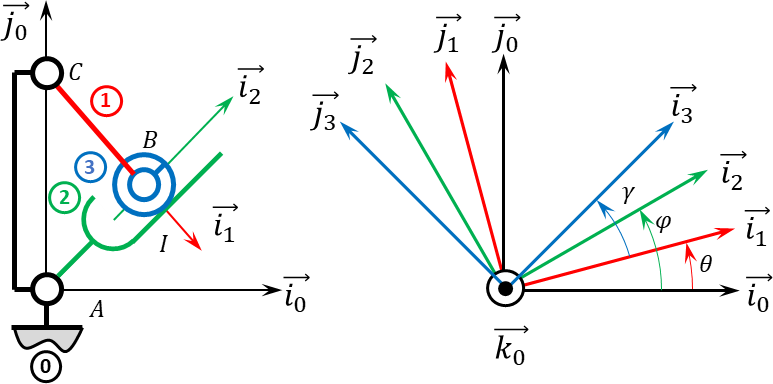
\includegraphics[width=\linewidth]{15_01}
\end{marginfigure}
\fi


Il est possible de mettre la loi entrée-sortie sous la forme *** (voir exercice \ref{C2:06:14}).

\question{En utilisant la condition de roulement sans glissement au point $I$, déterminer $\gamma(t)$ et $\dot{\gamma}(t)$.}
\ifprof
\else
\fi

\question{Donner le torseur cinématique $\torseurcin{V}{3}{2}$ au point $B$.}
\ifprof
\else
\fi


\ifprof
\else

\marginnote{Corrigé voir \ref{DYN:04:B2:12:14}.}

\fi